\section{System Architecture and Design}
\label{ch:design}

\subsection{Overall System Architecture}
Each node is a single operating-system process. Its \texttt{asyncio} event loop runs, on one thread, discovery (a HELLO every 3\,s, a 10\,s timeout), link-state gossip (every 5\,s), the receive path, the priority-ordered sender, the store-and-forward flush (every 10\,s) and the API server. All of them reach the network only through the \texttt{Transport} interface (Figure~\ref{fig:arch}). Because the shared state (neighbour table, mesh graph, map of packets awaiting an ACK) is touched by one thread only, no locks are needed and data races cannot occur.
\begin{figure}[!htbp]
\centering
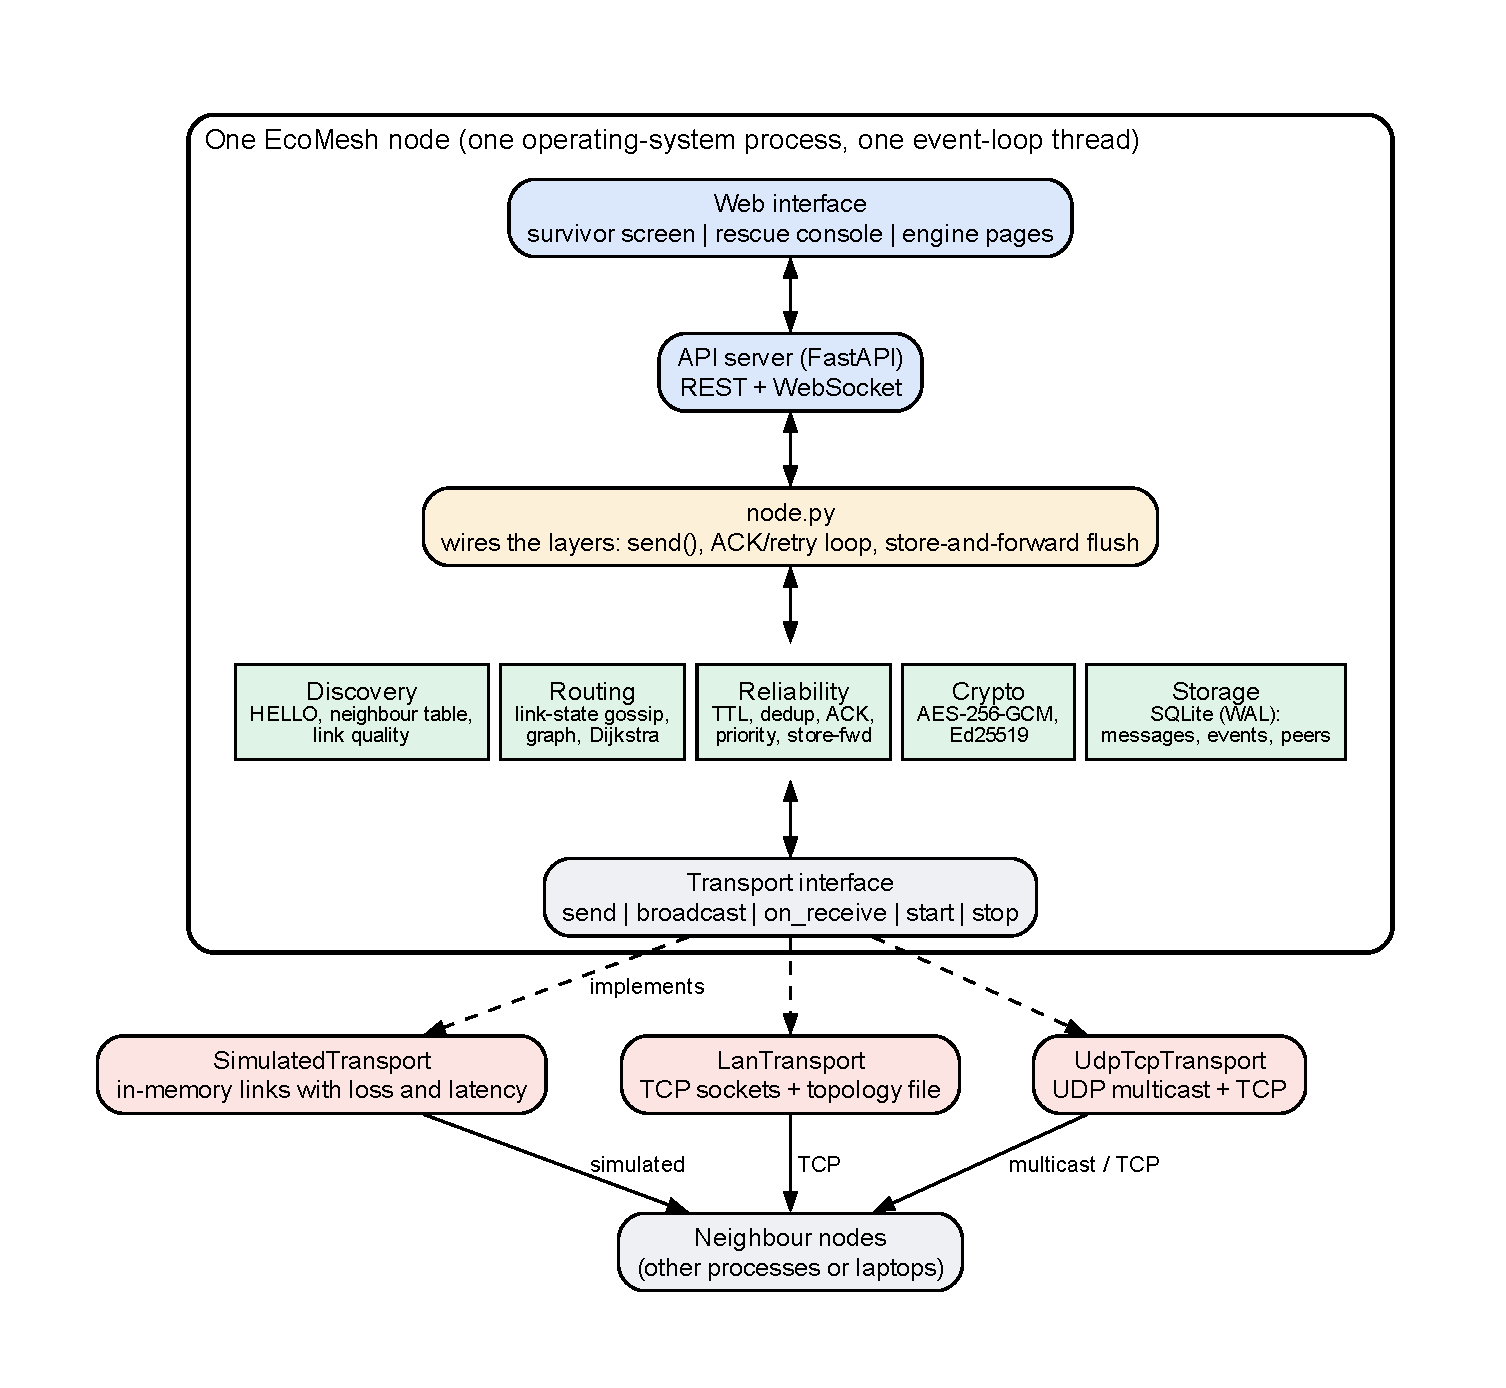
\includegraphics[width=0.72\textwidth]{figures/fig_architecture.pdf}
\caption{Block diagram: one EcoMesh node and its three interchangeable transports}
\label{fig:arch}
\end{figure}

\subsection{Component and Module Description}
The engine has one module per concern: \texttt{packet.py} (wire format), the transports, \texttt{discovery.py}, \texttt{routing.py}, \texttt{relay.py}, \texttt{reliability.py}, \texttt{crypto.py} and \texttt{store.py}, joined only in \texttt{node.py}. \texttt{sim/} and \texttt{api/} drive the engine for experiments, and \texttt{story/} serves the device screens. Table~\ref{tab:impl} in Section~\ref{sec:modules} gives each module's input and output, logic, dependencies and tests.

\textbf{Wire protocol.} A fixed big-endian header (Table~\ref{tab:header}) is followed by the path travelled so far, the payload and an optional 64-byte signature. The path is carried so that loops can be detected and the screens can show the route. HELLO is a one-hop broadcast, LINK\_STATE is sent to each neighbour, and DATA and ACK travel over TCP on each hop, so every hop is ordered and reliable even though the end-to-end path is not.
\begin{table}[!htbp]
\caption{The 52-byte packet header}
\label{tab:header}
\footnotesize
\setlength{\tabcolsep}{3.5pt}
\begin{tabular}{@{}rrll@{\hspace{8pt}}rrll@{}}
\toprule
\textbf{Off.} & \textbf{Size} & \textbf{Field} & \textbf{Meaning} & \textbf{Off.} & \textbf{Size} & \textbf{Field} & \textbf{Meaning}\\ \midrule
0 & 2 & magic & \texttt{0x4D45} ``ME'' & 24 & 8 & src & node id, ASCII\\
2 & 1 & version & 1 & 32 & 8 & dst & node id / \texttt{RESCUE\_\_}\\
3 & 1 & type & HELLO, LINK\_STATE, DATA, ACK & 40 & 8 & timestamp & Unix ms\\
4 & 1 & priority & 0 SOS, 1 NORMAL, 2 STATUS & 48 & 2 & payload\_len & bytes\\
5 & 1 & ttl & per-hop decrement (10) & 50 & 1 & path\_len & ids in path\\
6 & 1 & flags & enc., needs\_ack, s-f, signed & 51 & 1 & attempt & retry counter\\
7 & 1 & hop\_count & per-hop increment & 8 & 16 & msg\_id & UUIDv4\\
\bottomrule
\end{tabular}
\end{table}

\subsection{Architecture Selection and Justification}
\textbf{Layered and independent of the transport.} A single boundary separates moving bytes from everything else, which gives a deterministic simulator, unit tests without sockets and a direct answer to the missing radio: a Bluetooth transport would be one more implementation, not a rewrite. \textbf{One \texttt{asyncio} thread instead of several threads.} Four activities share three structures; on one loop they cannot race, so correctness does not depend on locking discipline. \textbf{Peer-to-peer instead of client--server.} A server would be a single point of failure and exactly the infrastructure that fails in a disaster. \textbf{Link state instead of flooding or on-demand discovery.} Flooding breaks down under load, and discovering a route on demand delays the first emergency packet. \textbf{SQLite per node in WAL mode.} It is a file with no server, and the API can read while the engine writes.

\subsection{Data Flow Diagram (DFD)}
Figure~\ref{fig:dfd0} is the context diagram (one node, no server); Figure~\ref{fig:dfd1} splits the node into six processes and five data stores.
\begin{figure}[!htbp]
\centering
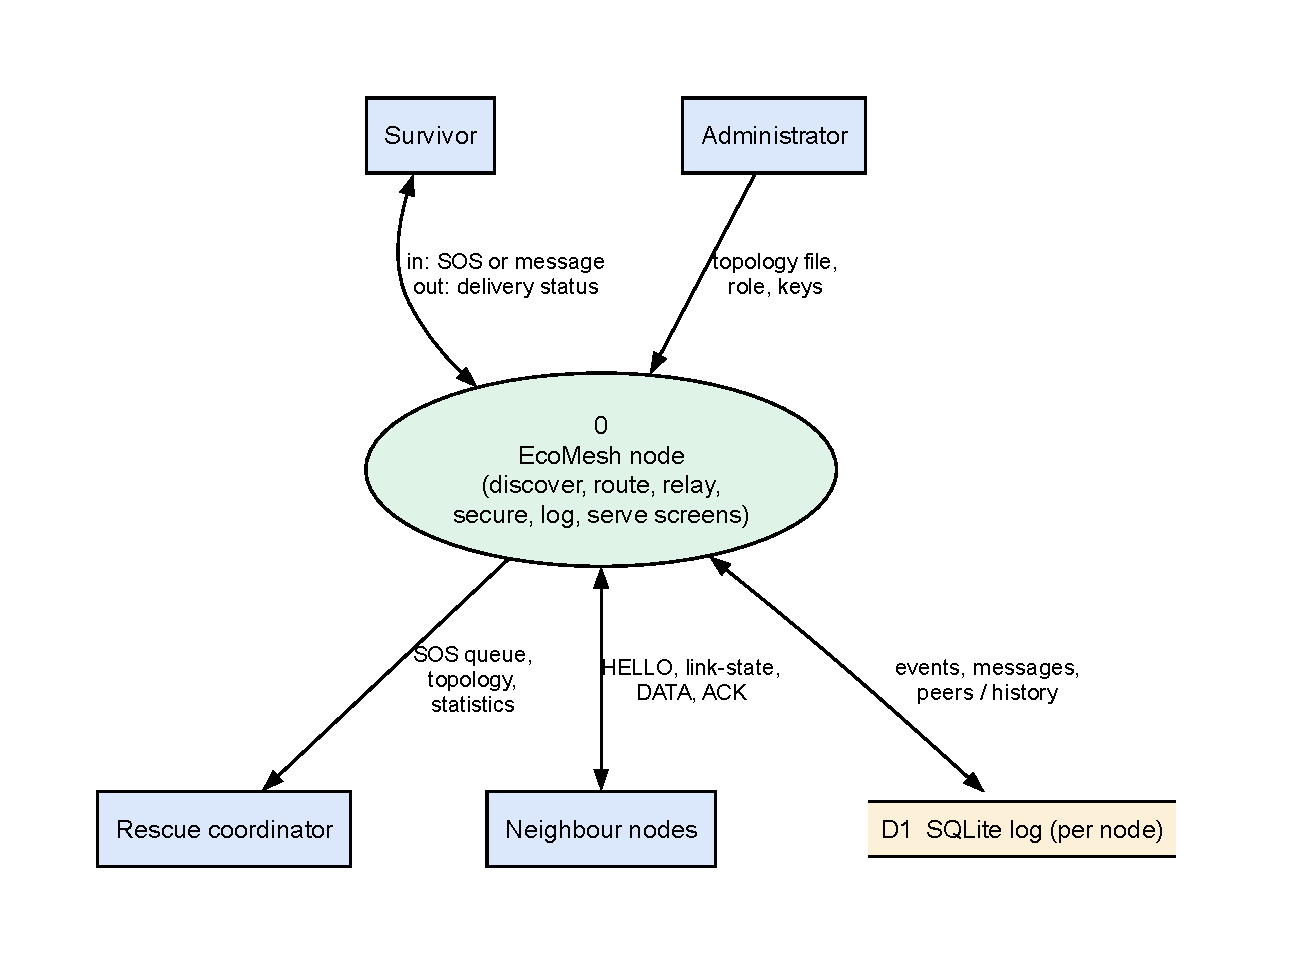
\includegraphics[width=0.5\textwidth]{figures/fig_dfd0.pdf}
\caption{Level-0 (context) data flow diagram}
\label{fig:dfd0}
\end{figure}
\begin{figure}[!htbp]
\centering
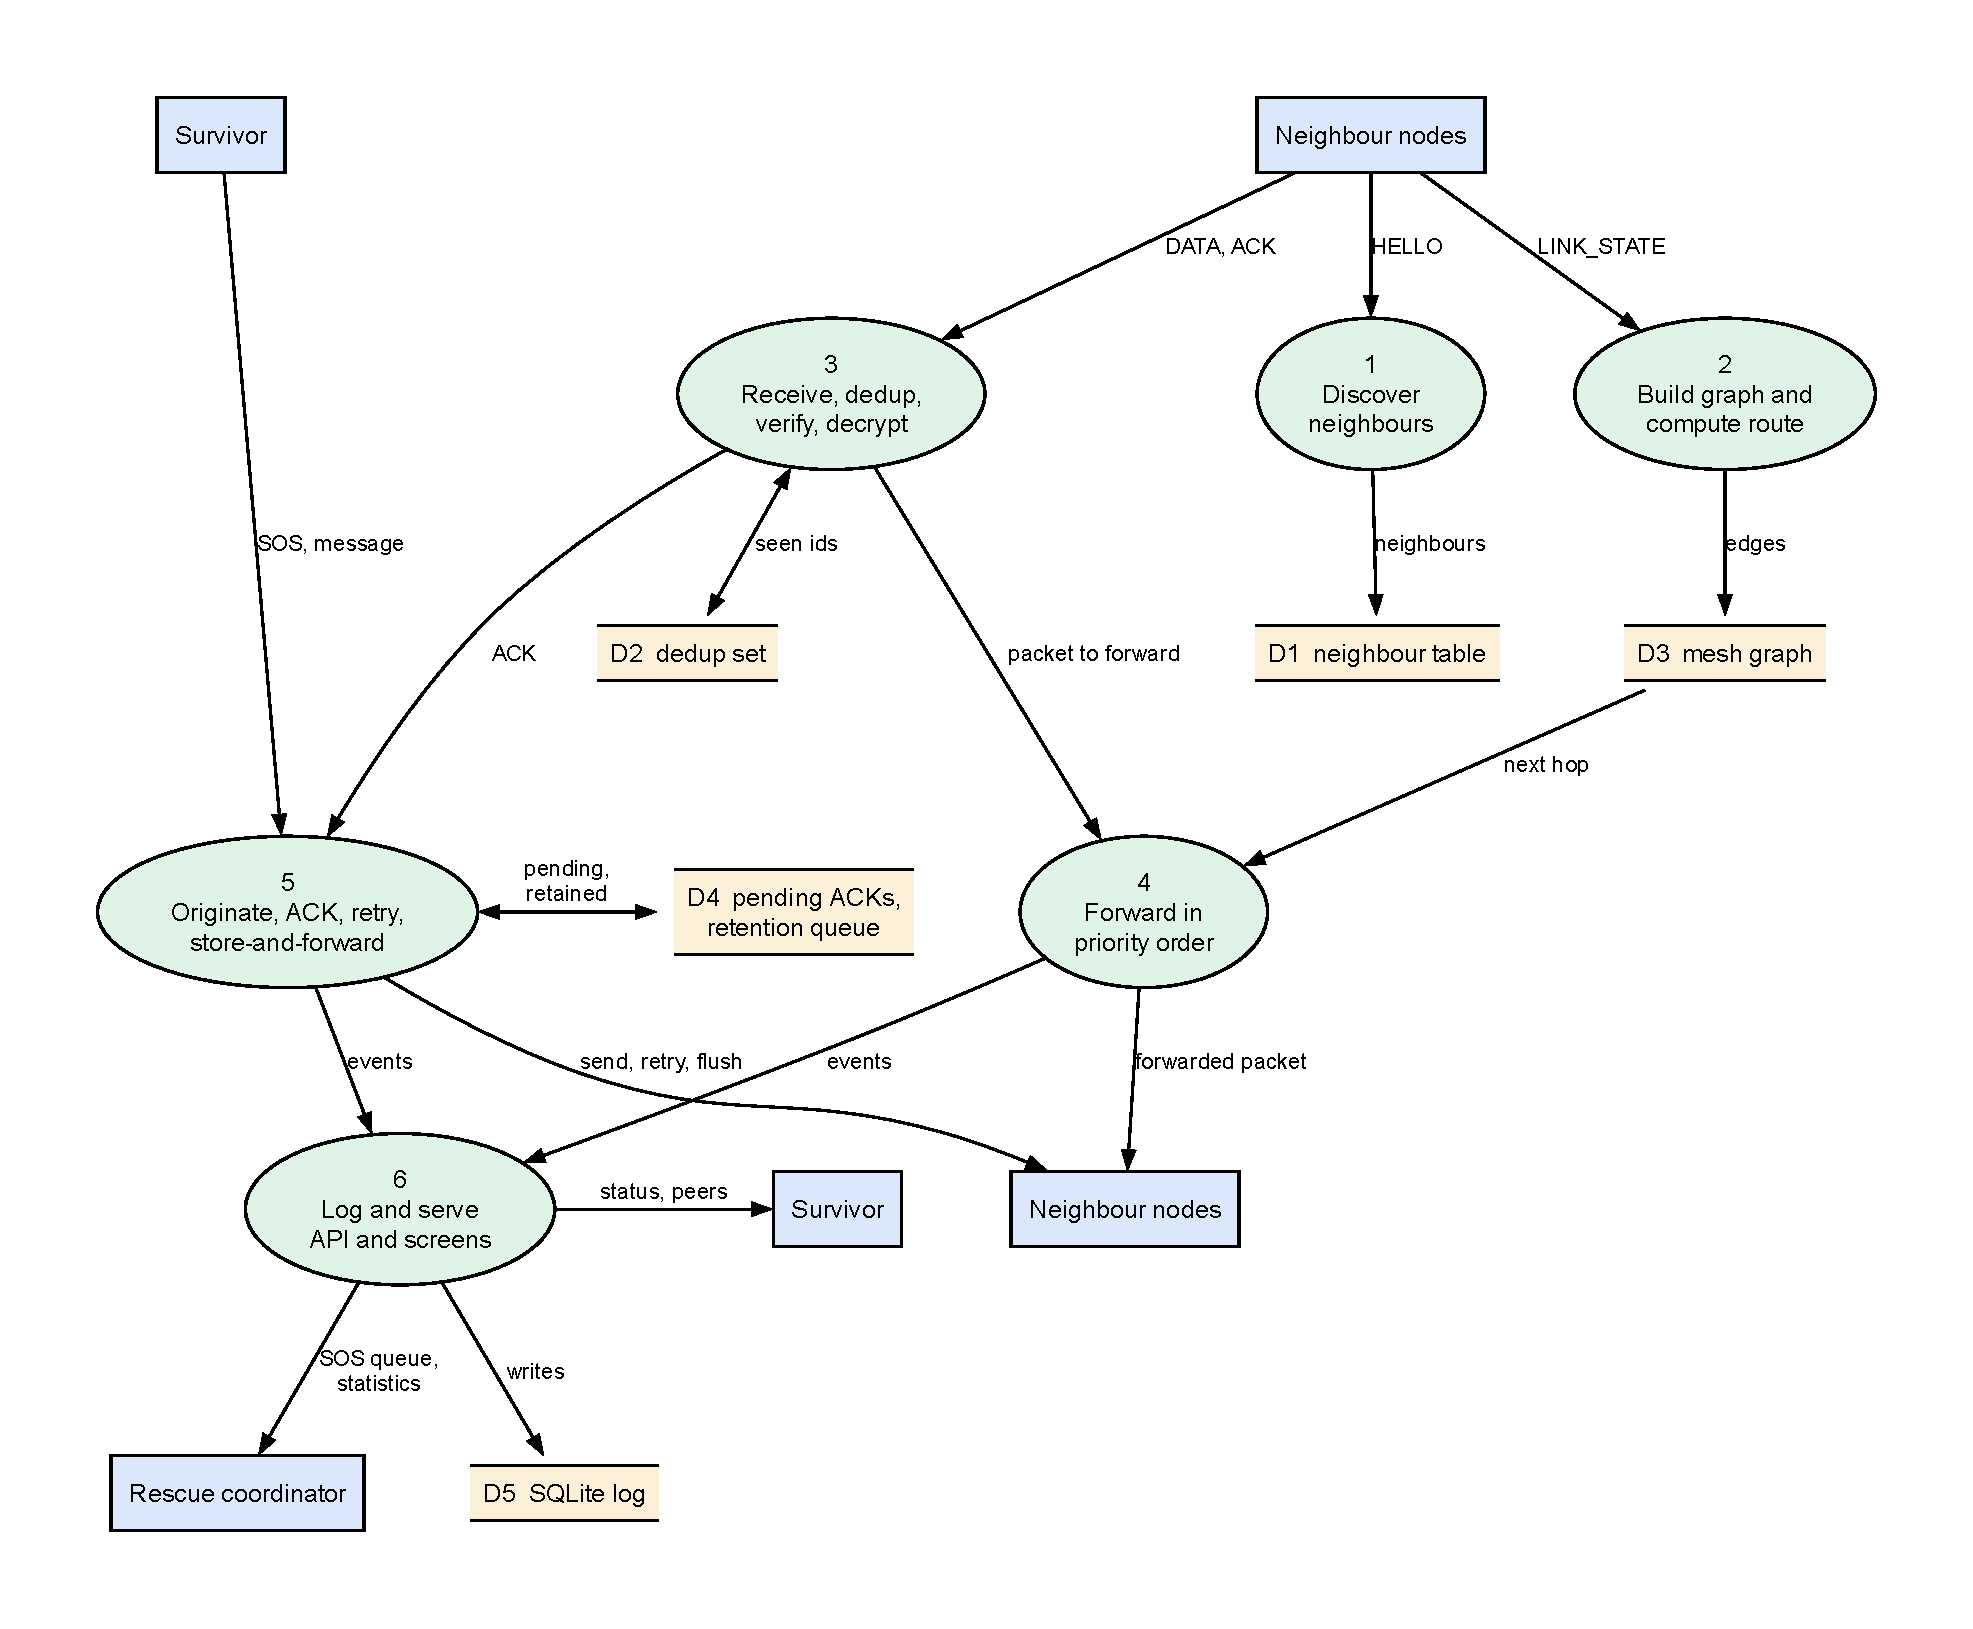
\includegraphics[width=\textwidth,height=0.52\textheight,keepaspectratio]{figures/fig_dfd1.pdf}
\caption{Level-1 data flow diagram of one node}
\label{fig:dfd1}
\end{figure}

\subsection{UML Diagrams}
The six UML diagrams of Phase~II match the implemented design. \textbf{Use case diagram} (Figure~\ref{fig:usecase}): five actors; raising an SOS includes sending a message, and holding and flushing extends sending when there is no route.
\begin{figure}[!htbp]
\centering
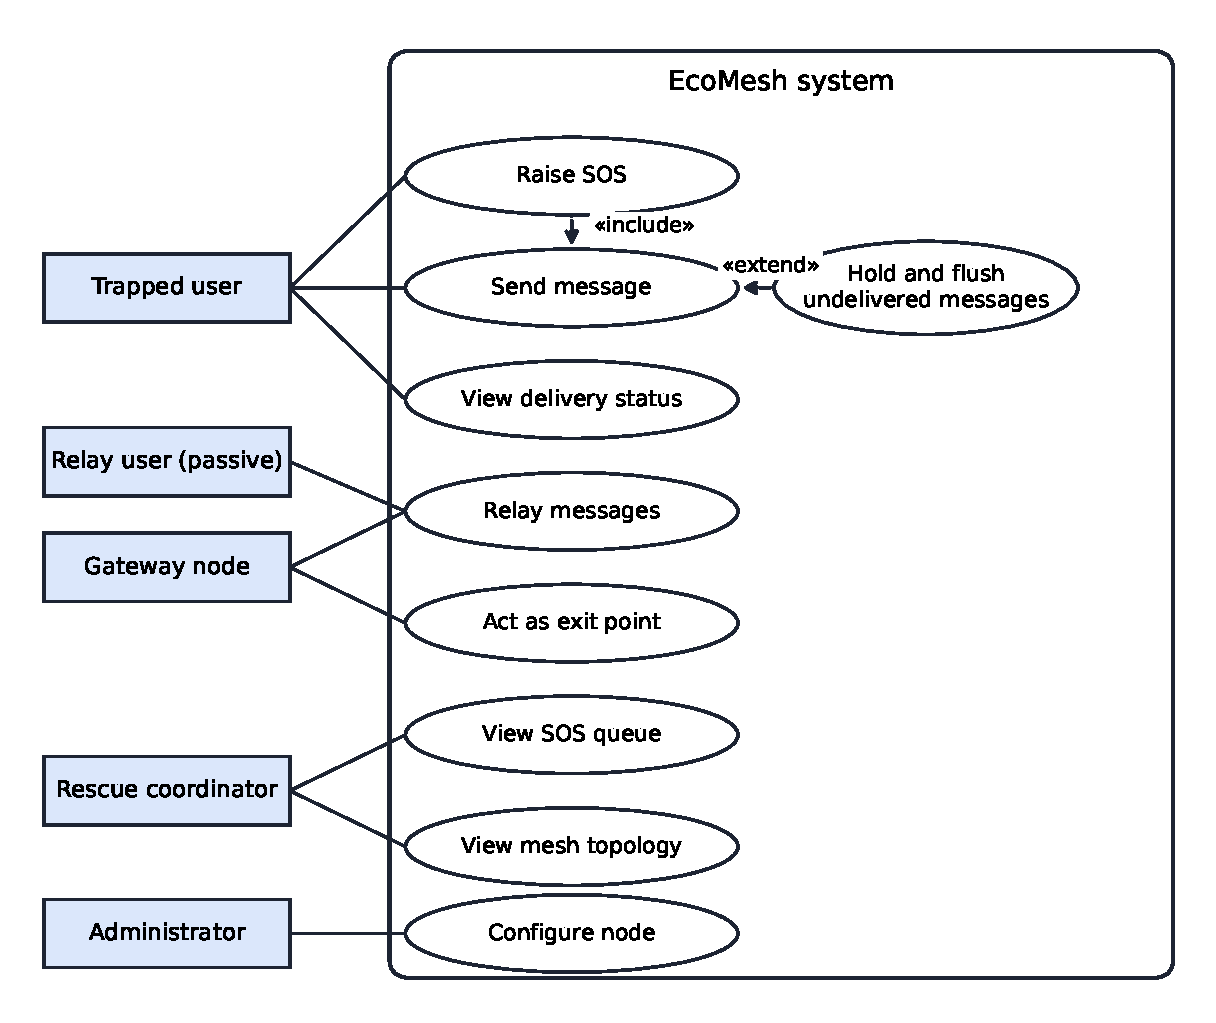
\includegraphics[width=0.62\textwidth]{figures/uml_usecase.pdf}
\caption{Use case diagram}
\label{fig:usecase}
\end{figure}
\textbf{Class diagram} (Figure~\ref{fig:class}). \texttt{Node} owns the discovery, gossip, routing, relay, ACK-tracking, retention and storage objects (filled diamonds); the router and the gossip share one \texttt{MeshGraph}; the relay owns its priority queue and uses a duplicate set; three classes implement \texttt{Transport}. \textbf{Activity diagram} (Figure~\ref{fig:activity}). An arriving packet is validated and checked for duplicates. If it is addressed to this node, its signature is verified and its payload decrypted, and it is logged, acknowledged and delivered; otherwise the TTL, loop and route checks decide whether it is dropped or queued again by priority.
\begin{figure}[!htbp]
\centering
\begin{minipage}[b]{0.49\textwidth}\centering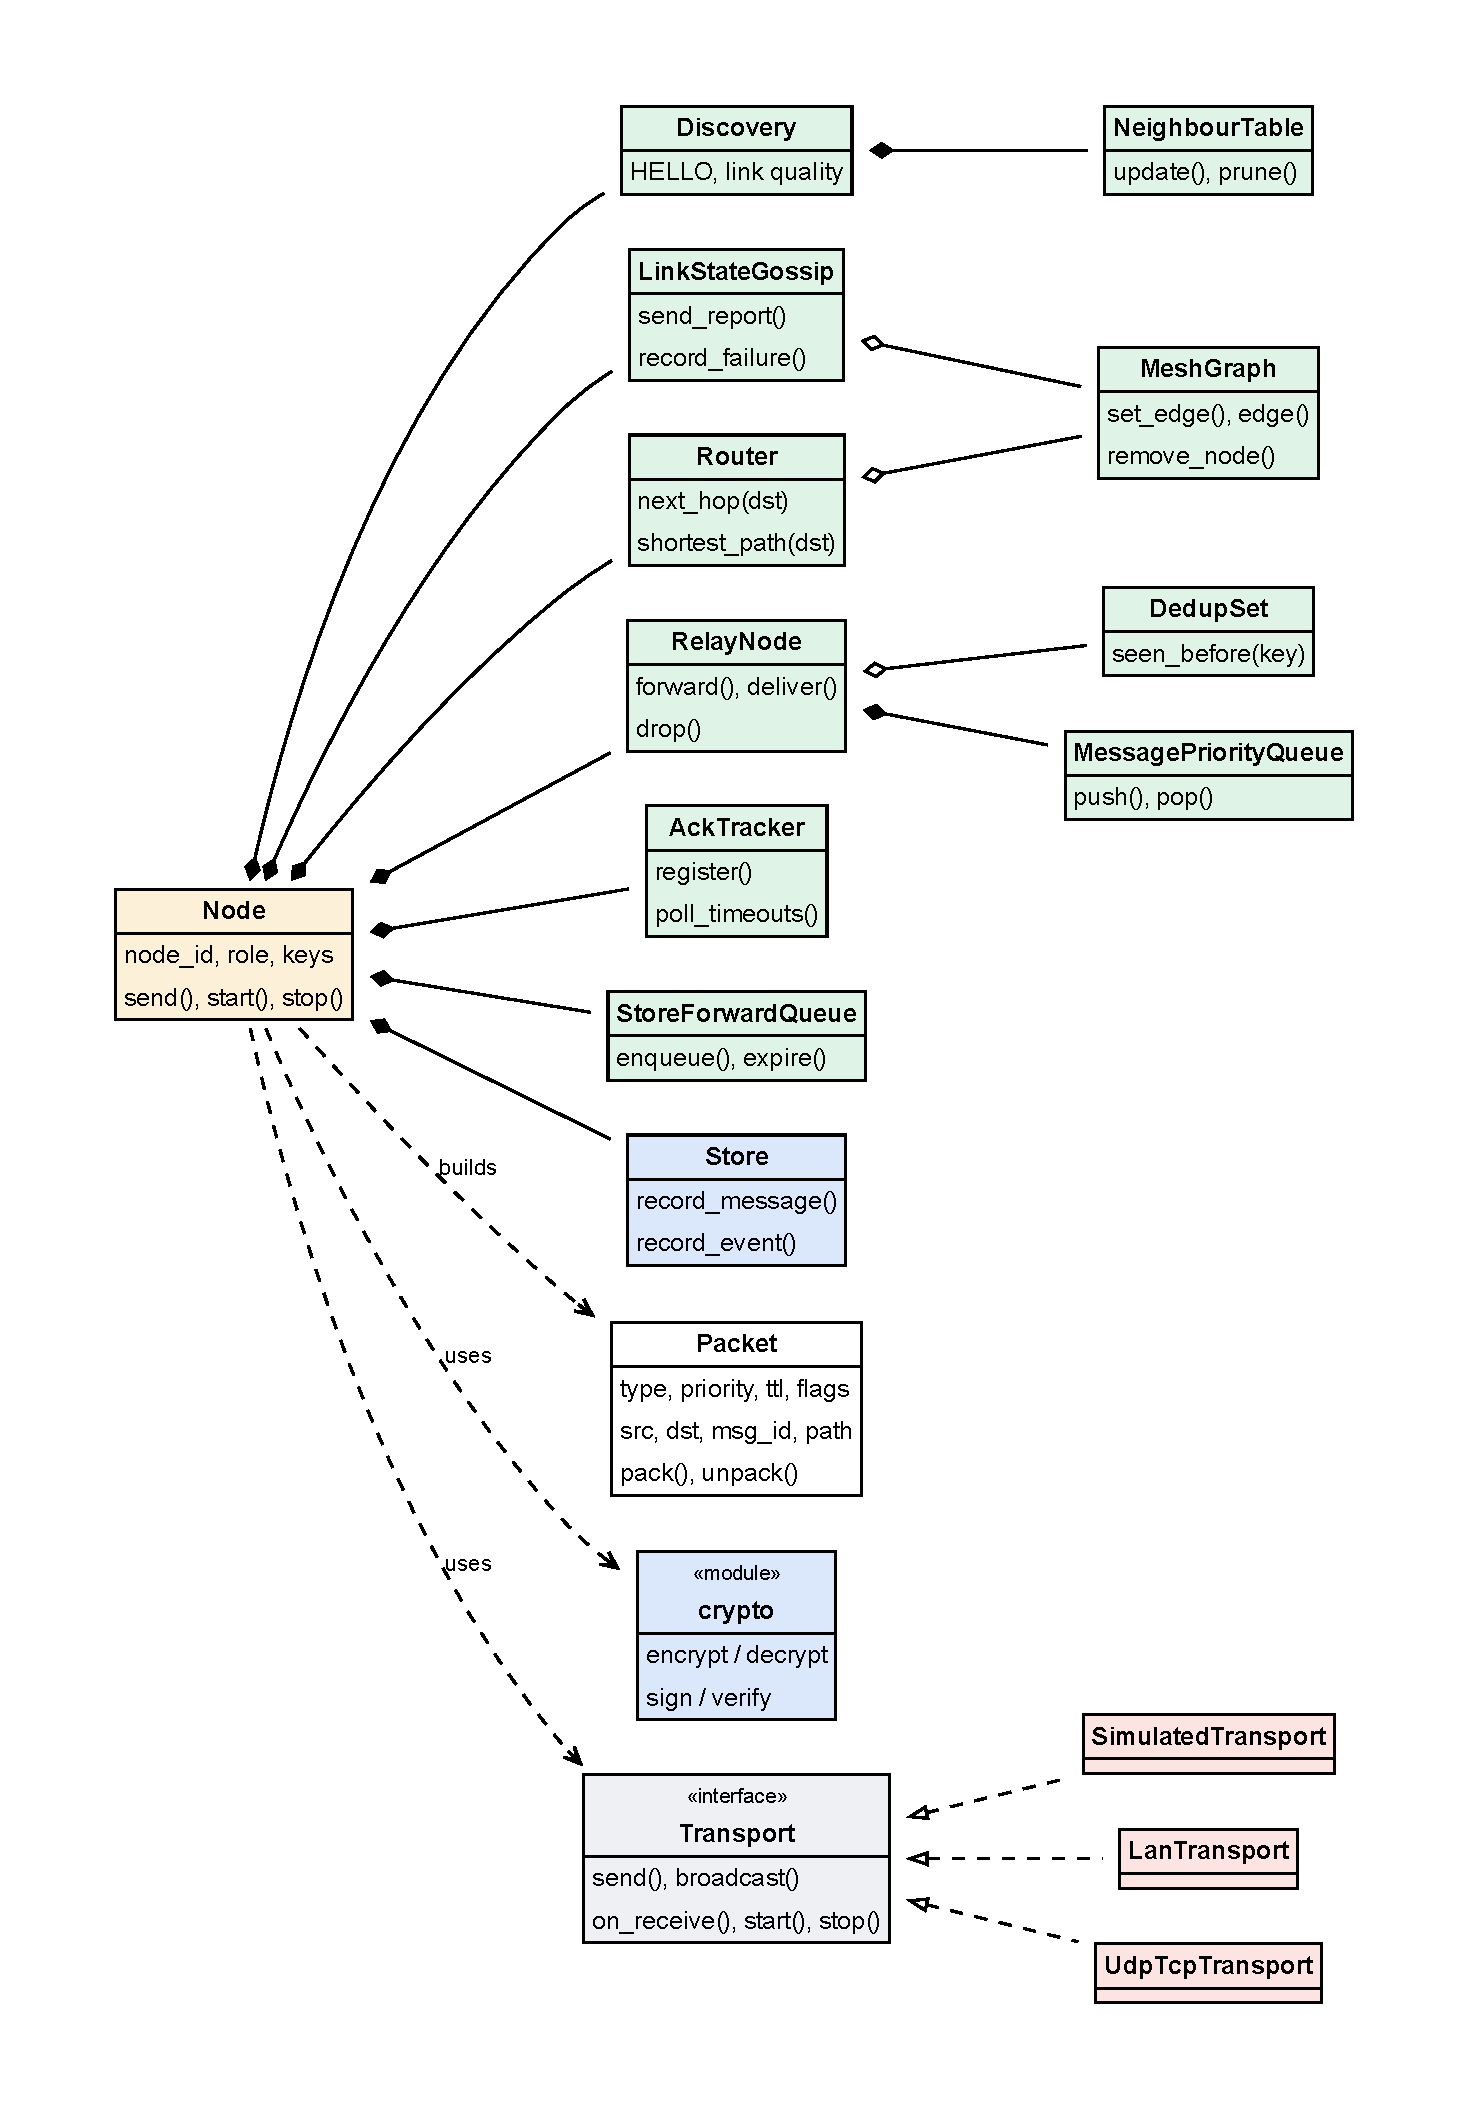
\includegraphics[width=\linewidth,height=0.49\textheight,keepaspectratio]{figures/uml_class.pdf}
\captionof{figure}{Class diagram: \texttt{Node} as the composition root}\label{fig:class}\end{minipage}\hfill
\begin{minipage}[b]{0.49\textwidth}\centering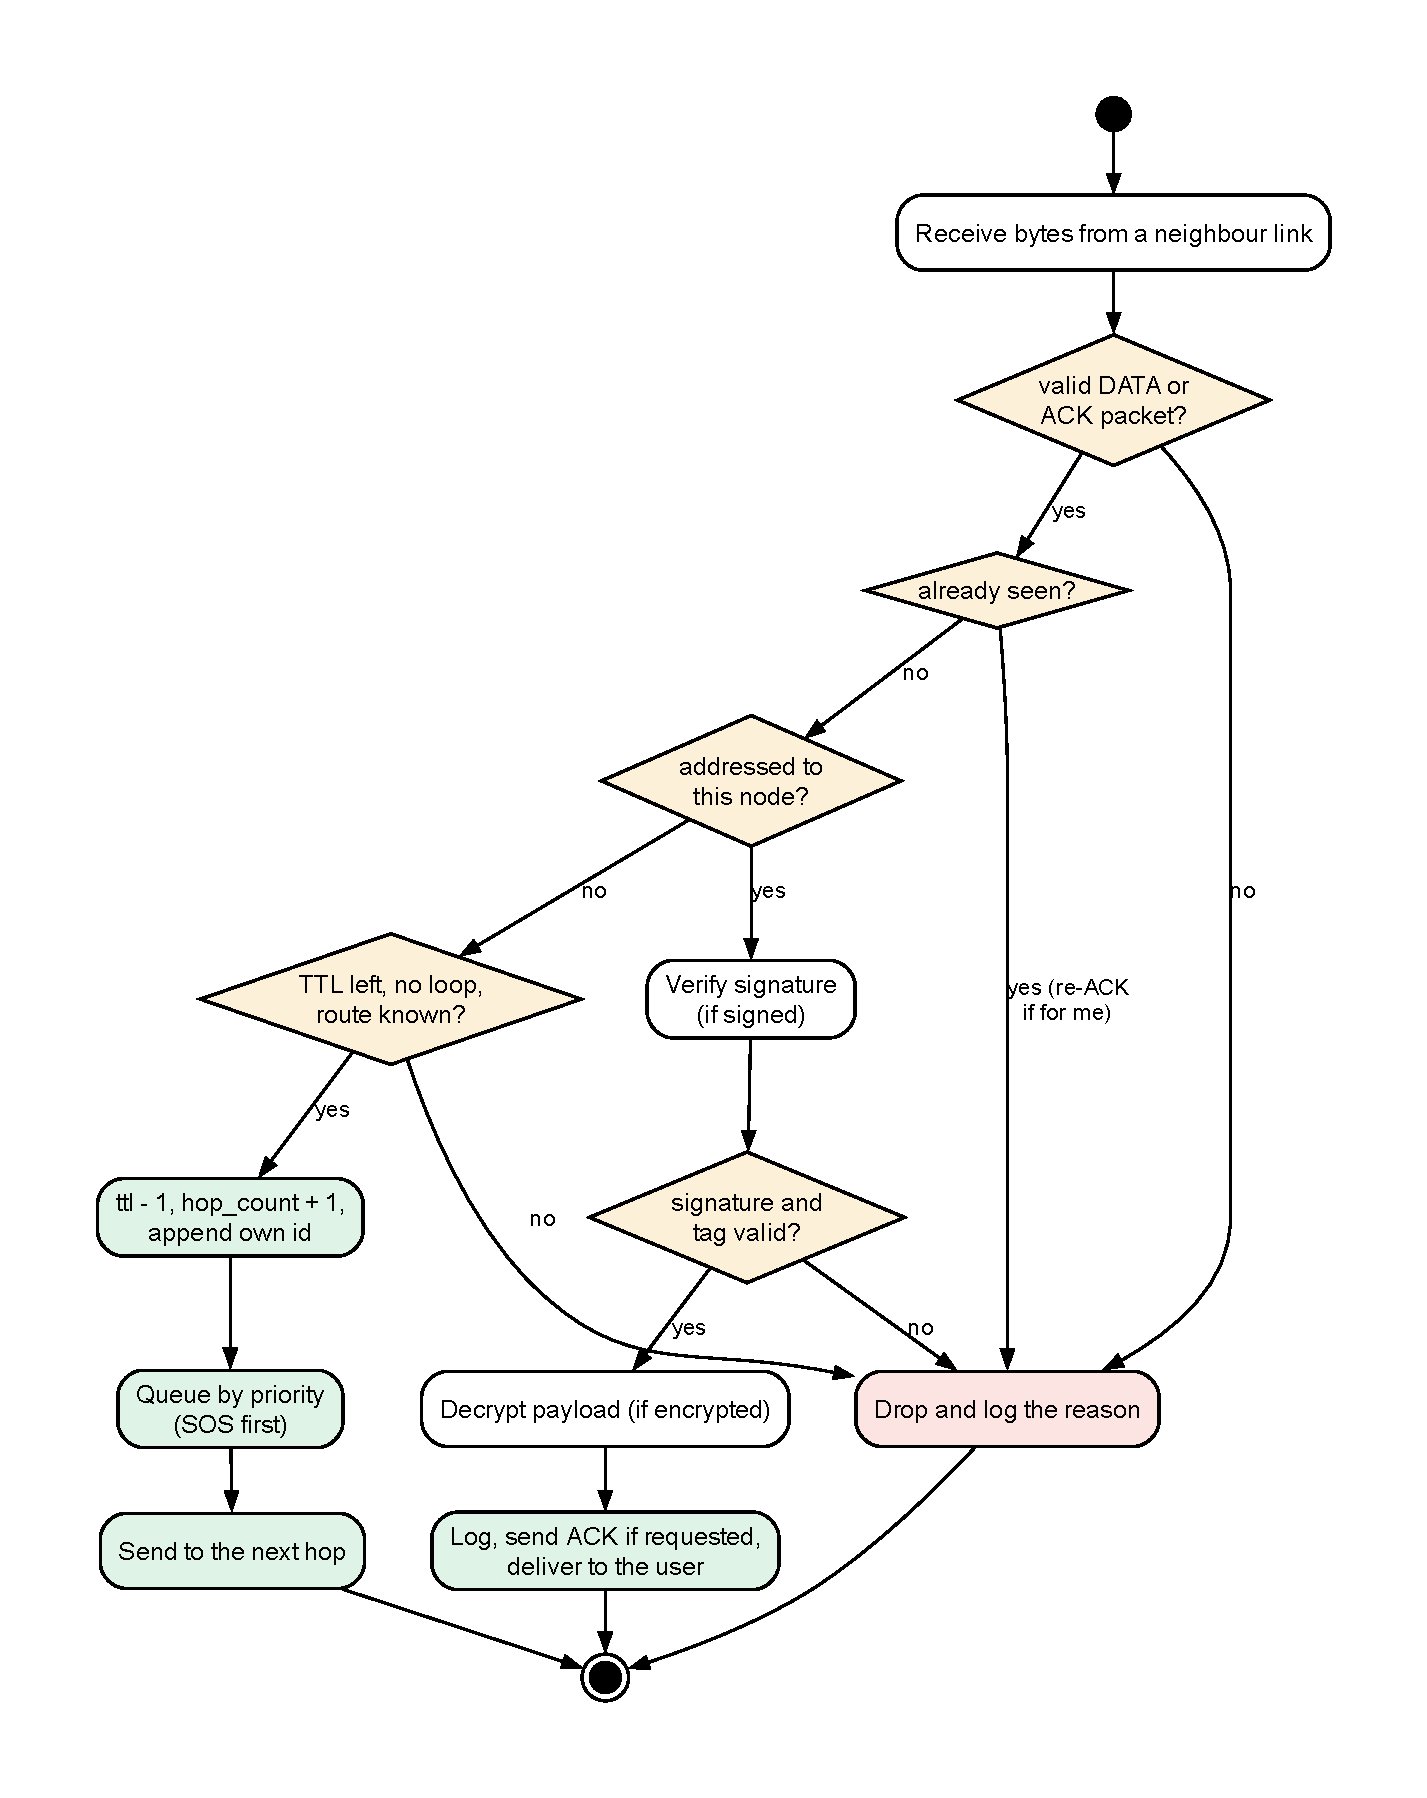
\includegraphics[width=\linewidth,height=0.49\textheight,keepaspectratio]{figures/uml_activity.pdf}
\captionof{figure}{Activity diagram: the packet receive path}\label{fig:activity}\end{minipage}
\end{figure}
\textbf{Sequence diagram} (Figure~\ref{fig:sequence}). L1 creates, encrypts and signs an SOS; each relay checks duplicates, lowers the TTL and adds its id; L5 delivers it and the ACK returns.
\begin{figure}[!htbp]
\centering
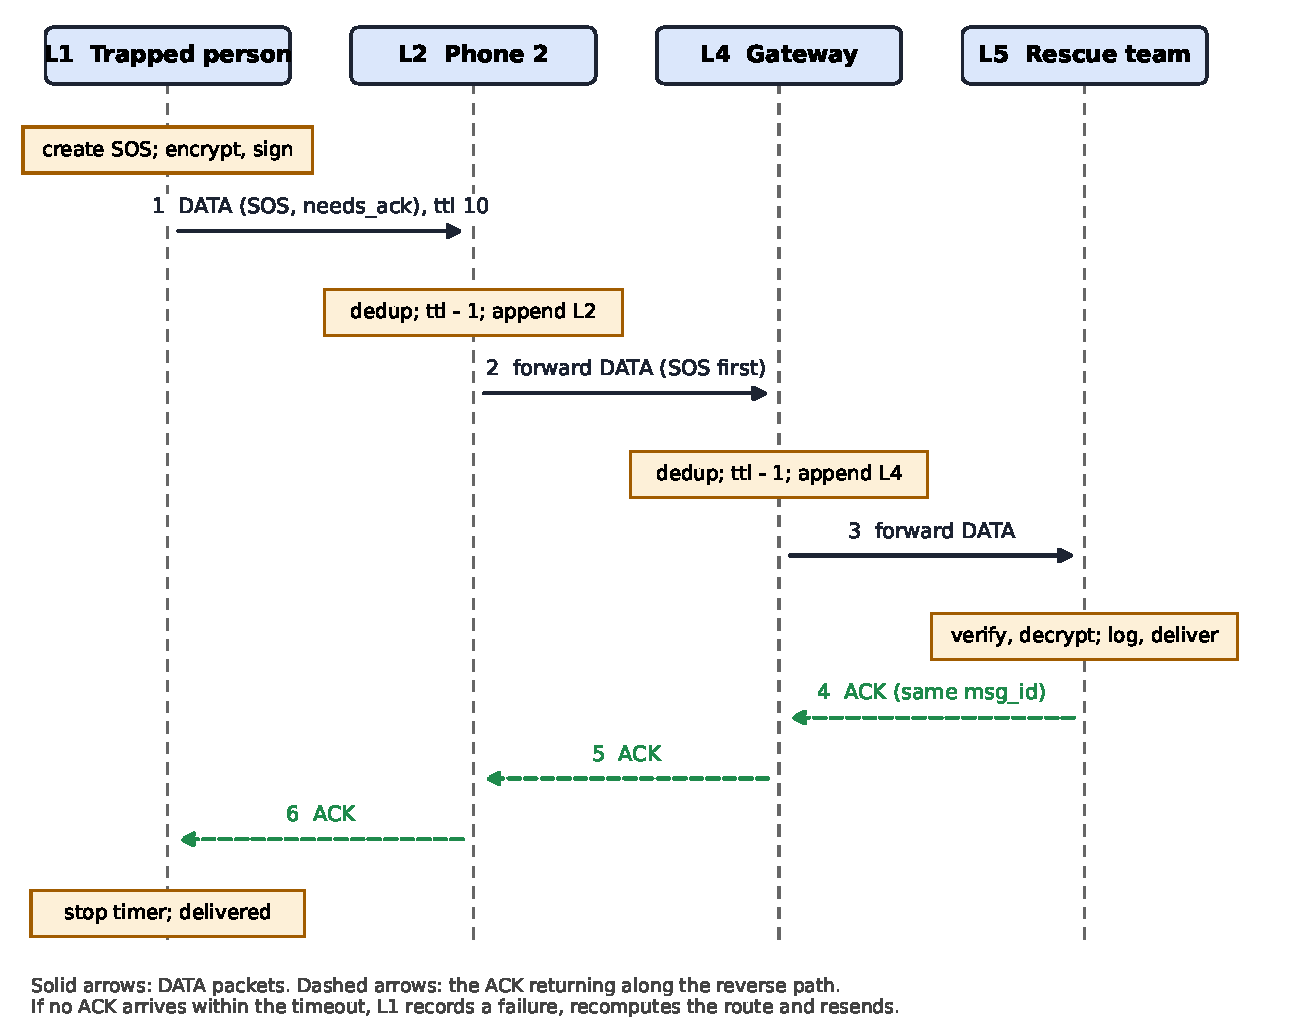
\includegraphics[width=0.82\textwidth]{figures/uml_sequence.pdf}
\caption[Sequence diagram: an SOS relayed hop by hop]{Sequence diagram: an SOS relayed hop by hop with the ACK returning along the reverse path}
\label{fig:sequence}
\end{figure}
\textbf{State machine} (Figure~\ref{fig:state}, left). A message is created, becomes pending (sent and awaiting an ACK) or held (no route), and ends delivered or failed; these states are the \texttt{status} values stored in the database. \textbf{Deployment diagram} (Figure~\ref{fig:deploy}, right). Five node processes, each with its own engine, web screen and SQLite file, connected only by the TCP links that the topology file lists; there is no server (Section~\ref{sec:lan}).
\begin{figure}[!htbp]
\centering
\begin{minipage}[b]{0.52\textwidth}\centering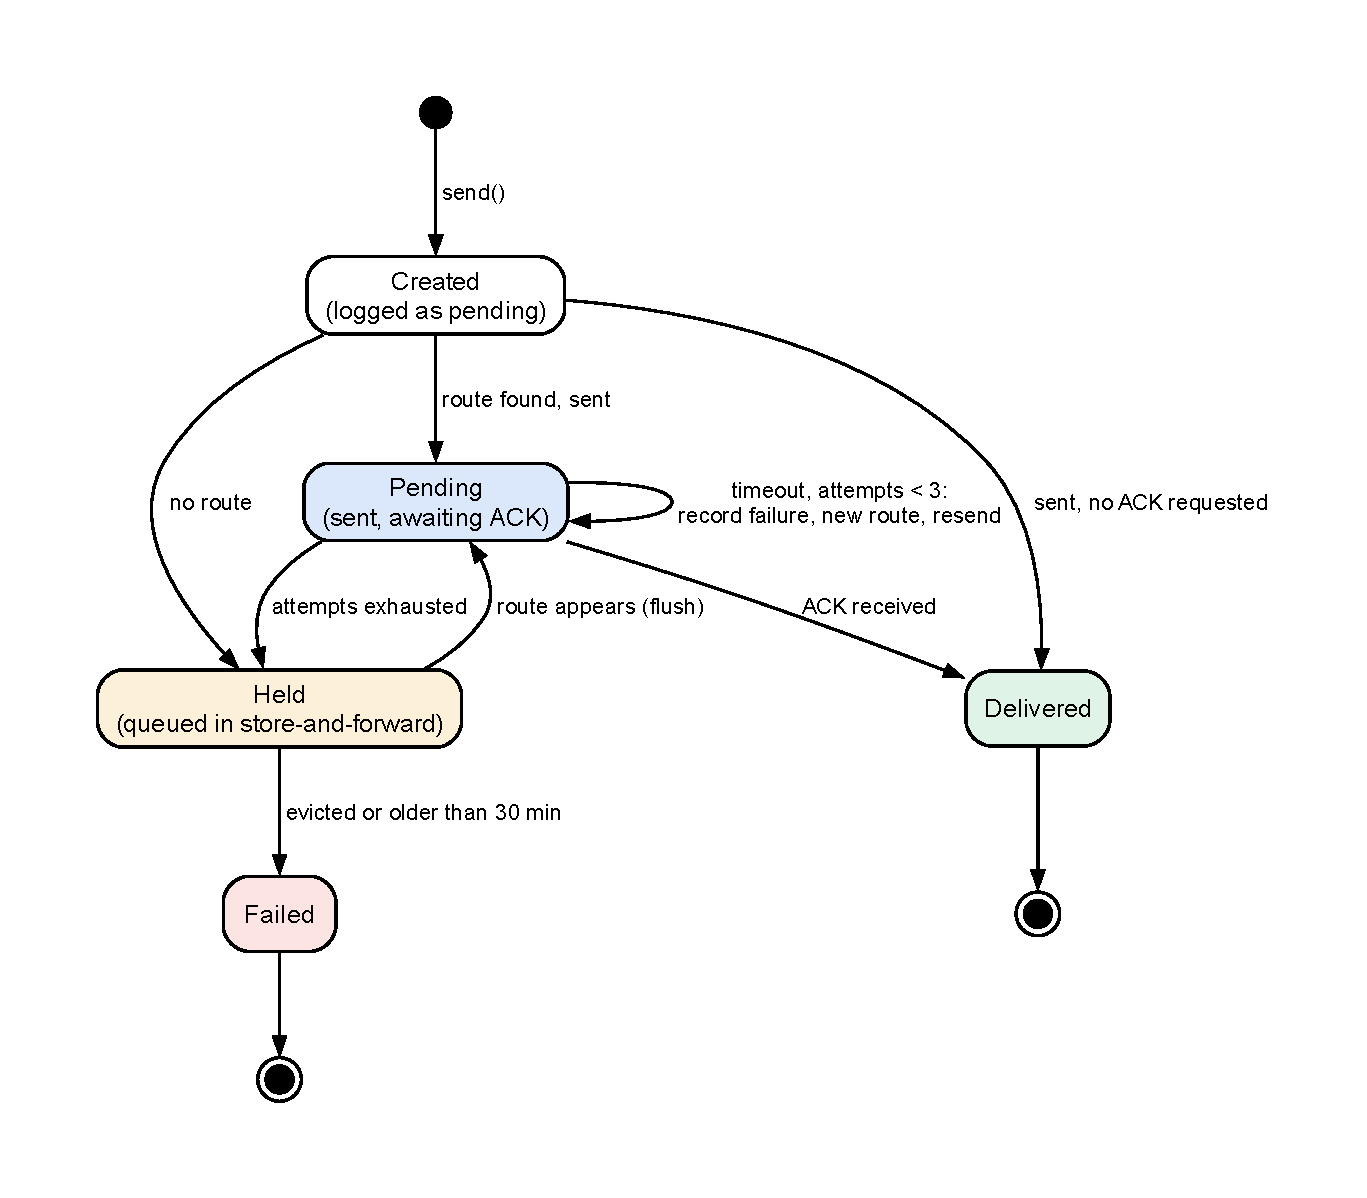
\includegraphics[width=\textwidth]{figures/uml_state.pdf}\end{minipage}\hfill
\begin{minipage}[b]{0.36\textwidth}\centering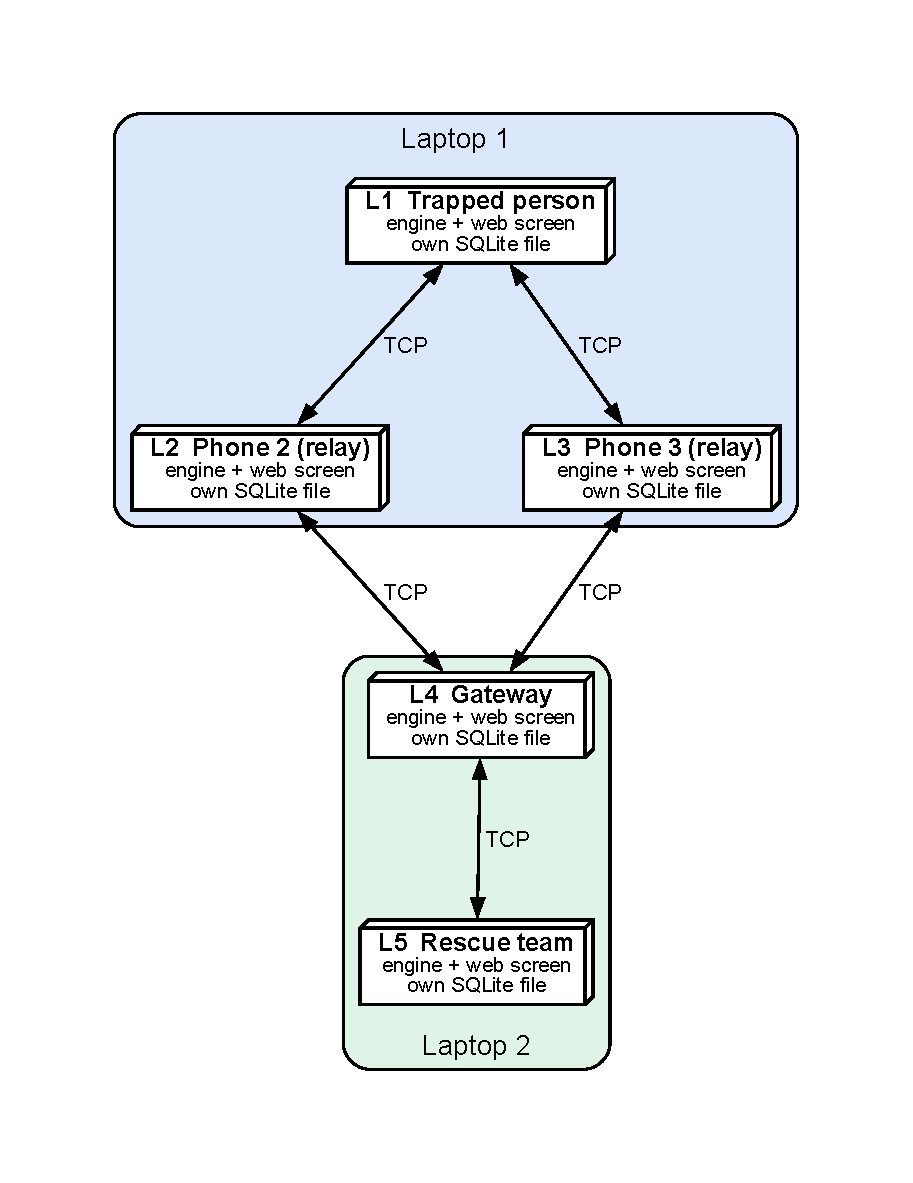
\includegraphics[width=\textwidth]{figures/uml_deploy.pdf}\end{minipage}
\caption[State machine of the message lifecycle and deployment diagram]{State machine of the message lifecycle (left) and deployment diagram of the live configuration (right)}
\label{fig:state}\label{fig:deploy}
\end{figure}

\subsection{Database Design}
\label{sec:db}
Every node keeps its own SQLite database in WAL mode, accessed with plain \texttt{sqlite3} and SQL; with only three tables an ORM would add indirection and nothing else. Every metric is a query over this database (SRS 6.1).
\begin{figure}[!htbp]
\centering
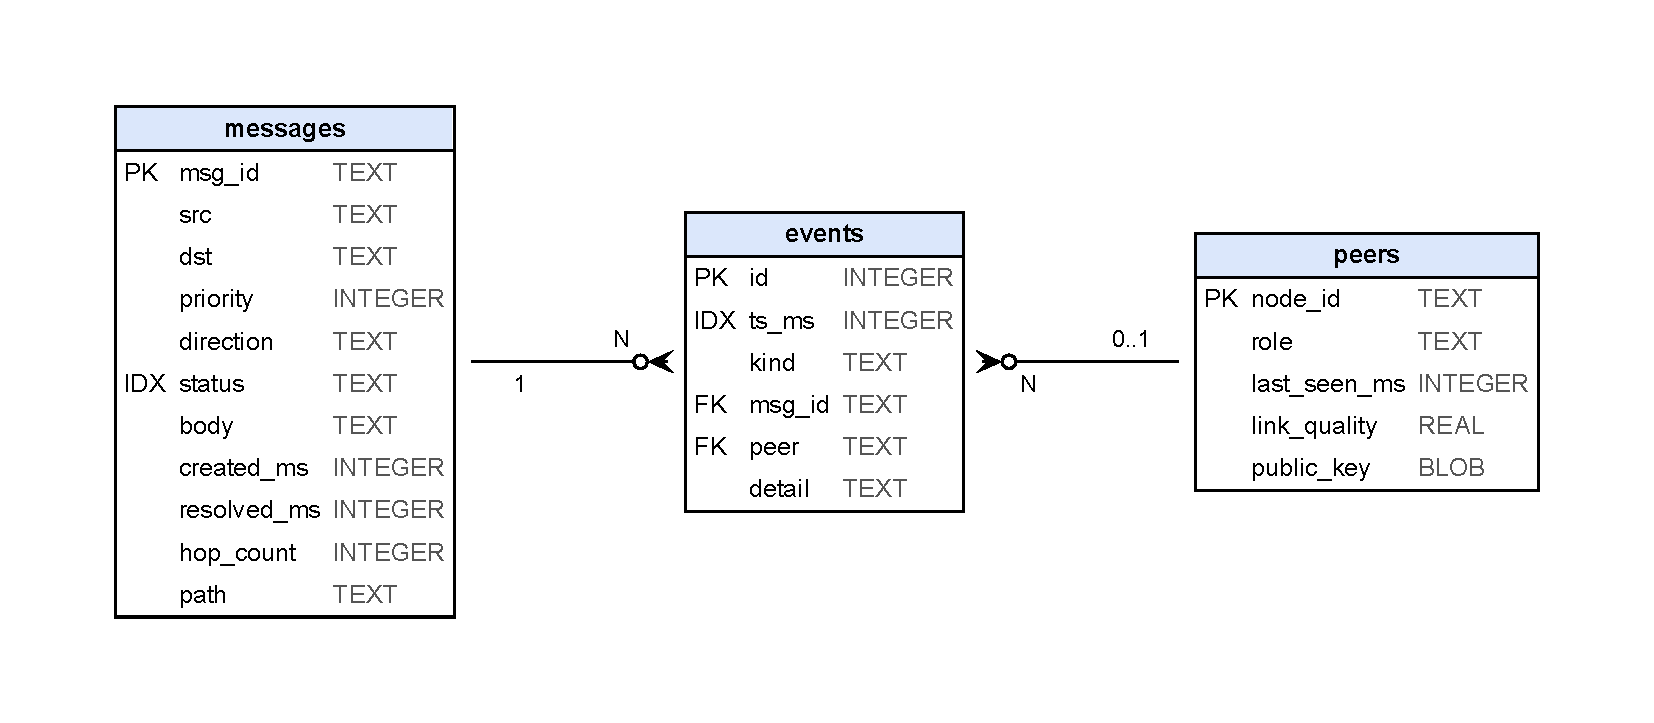
\includegraphics[width=0.92\textwidth]{figures/fig_er.pdf}
\caption[Entity--relationship diagram of the per-node database]{Entity--relationship diagram of the per-node database (PK primary key, IDX secondary index, FK logical foreign key)}
\label{fig:er}
\end{figure}
\textbf{Relational schema.} \texttt{messages}(\texttt{msg\_id} PK, \texttt{src}, \texttt{dst}, \texttt{priority}, \texttt{direction} in sent/received/forwarded, \texttt{status} in pending/delivered/failed/queued\_sf, \texttt{body}, \texttt{created\_ms}, \texttt{resolved\_ms}, \texttt{hop\_count}, \texttt{path}); \texttt{events}(\texttt{id} PK, \texttt{ts\_ms}, \texttt{kind}, \texttt{msg\_id}, \texttt{peer}, \texttt{detail}); \texttt{peers}(\texttt{node\_id} PK, \texttt{role}, \texttt{last\_seen\_ms}, \texttt{link\_quality}, \texttt{public\_key}). \textbf{Keys and integrity.} The UUID \texttt{msg\_id} joins messages to events; \texttt{body} holds plaintext only at source and destination; upserts move a message from pending to queued\_sf to delivered in one row; \texttt{events.msg\_id} and \texttt{events.peer} are logical foreign keys, since a relay logs events for messages it never stores. \textbf{Normalisation.} Third normal form, except the comma-separated \texttt{path}, always read whole. \textbf{Indexing.} \texttt{idx\_events\_ts} serves the live panel and \texttt{idx\_msg\_status} the held-message count. \textbf{Sample records} are in Table~\ref{tab:samples}; the relay's row has no body.
\begin{table}[htbp]
\caption{Sample rows of \texttt{messages} for one SOS from A to C in a real run: each node holds its own view of the same message id}
\label{tab:samples}
\footnotesize
\setlength{\tabcolsep}{3pt}
\begin{tabular}{@{}llllllllll@{}}
\toprule
\textbf{DB} & \textbf{msg\_id} & \textbf{src} & \textbf{dst} & \textbf{prio} & \textbf{direction} & \textbf{status} & \textbf{body} & \textbf{hops} & \textbf{path} \\ \midrule
A & 8e859198... & A & C & 0 & sent & delivered & trapped on floor 3 & 1 & B \\
B & 8e859198... & A & C & 0 & forwarded & delivered & NULL & 1 & B \\
C & 8e859198... & A & C & 0 & received & delivered & trapped on floor 3 & 1 & B \\
\bottomrule
\end{tabular}
\end{table}


\subsection{Security and Error Handling Design}
\label{sec:secdesign}
Table~\ref{tab:threat} links each threat to its countermeasure and requirement.
\begin{table}[!htbp]
\caption{Threat model and countermeasures}
\label{tab:threat}
\footnotesize
\begin{tabularx}{\textwidth}{@{}>{\raggedright\arraybackslash}p{4.0cm}>{\raggedright\arraybackslash}X>{\raggedright\arraybackslash}p{2.6cm}@{}}
\toprule
\textbf{Threat} & \textbf{Mechanism} & \textbf{Requirement}\\ \midrule
Relay reads a message & AES-256-GCM payload; relays see only routing fields & SEC-1, 2, FWD-7\\
Relay modifies a message & GCM tag fails at the destination; dropped, logged & SEC-5\\
Relay forges an SOS & Ed25519 signature over the identity fields & SEC-3, 4, 6\\
Replay of a captured packet & dedup set keyed on message id (300\,s) & REL-3\\
Malformed or hostile bytes & strict validation; \texttt{PacketError}; drop & FWD-6\\
Endless circulation & TTL per hop; own id in the path is a loop & FWD-3, 5\\
Hand-rolled cryptography & only \texttt{cryptography}-library primitives & SEC-7\\
\bottomrule
\end{tabularx}
\end{table}
\textbf{Authentication.} A node's identity is its Ed25519 key pair, announced in HELLO and gossip. \textbf{Authorisation.} Only GATEWAY and RESCUE nodes accept \texttt{RESCUE\_\_} traffic; any node may relay but never decrypts or stores what it does not own. One pre-shared key covers the mesh, so a node holding it could read what it forwards; per-pair keys would prevent this (Section~\ref{sec:limits}). \textbf{Input validation and exceptions.} Every field is range-checked; a violation raises \texttt{PacketError} and the packet is dropped and logged, never raised into the event loop; \texttt{verify} returns \texttt{False} instead of raising. \textbf{Logging.} Each drop has its own event (\texttt{drop\_ttl}, \texttt{drop\_loop}, \ldots). \textbf{Sensitive data.} Fresh 12-byte nonces; plaintext only at the two ends; private keys never sent; the signature skips fields that change in transit (TTL, hops, path).
